\documentclass{scrartcl}

\usepackage[utf8]{inputenc}
\usepackage[T1]{fontenc}
\usepackage[ngerman]{babel}
\usepackage{amssymb}
\usepackage{amsmath}
\usepackage{mathtools}
\usepackage{graphicx}
\usepackage{framed}
\usepackage{xcolor}
\usepackage[nottoc]{tocbibind}
\usepackage{caption}

\colorlet{shadecolor}{gray!25}
\setlength{\parindent}{0pt}

\newcommand{\abs}[1]{\left\lvert#1\right\rvert}


\begin{document}

\title{Lösen des Poisson-Problems mittels Finite-Differenzen-Diskretisierung\\
und CG-Verfahren}
\author{Marisa Breßler und Anne Jeschke (PPI27)}
\date{07.02.2020}
\maketitle

\tableofcontents

\pagebreak
\section{Motivation}
In unseren vorherigen Berichten haben wir das Poisson-Problem vorgestellt und einen numerischen Lösungsansatz aufgezeigt, der es durch eine Diskretisierung des Gebietes und des Laplace-Operators in das Lösen eines linearen Gleichungssystems überführt.
Die dabei entstehende tridiagonale Blockmatrix ist dünn besetzt, d.h. nur wenige Einträge sind ungleich Null.
Deswegen ist es sinnvoll, sie als sogenannte \textit{sparse}-Matrix abzuspeichern.
Dieser Speicherplatzvorteil geht jedoch beim Lösen des linearen Gleichungssystems mittels Gauß-Algorithmus und LU-Zerlegung verloren, da eine LU-Zerlegung einer dünn besetzten Matrix im Allgemeinen nicht dünn besetzt ist.
Aufgrund dieses Umstandes erscheint es sinnvoll, das lineare Gleichungssystem nicht direkt, sondern iterativ zu lösen.
Solche iterativen Lösungsverfahren (wie das Gesamtschrittverfahren von Jacobi, das Einzelschrittverfahren von Gauß-Seidel, das SOR-Verfahren und das CG-Verfahren) bieten gegenüber direkten Verfahren außerdem den Vorteil, dass deren Rechenaufwand im Verhältnis zur in der Praxis für gewöhnlich sehr großen Dimension der Blockmatrix recht gering ist.
Da das CG-Verfahren eine heute durchaus übliche Methode zum Lösen großer linearer Gleichungssysteme darstellt, wollen wir dieses im Folgenden im Rahmen unseres bisherigen Settings (das Poisson-Problem für die Beispielfunktion aus unserem Bericht vom 03.01.2020 und einer Diskretisierung des Einheitsintervalls, -quadrats und -würfels mit finiten Differenzen) vorstellen und untersuchen.



\pagebreak
\section{Theoretische Grundlagen und Algorithmus}

Im Gegensatz zu den bisher behandelten direkten Verfahren, die nach einer endlichen Anzahl von Rechenschritten den Lösungsvektor $x$ des linearen Gleichungssystems $Ax=b$ mit $A\in\mathbb{R}^{N\times N}$ und $b\in\mathbb{R}^N$ liefern, definiert man bei den iterativen Verfahren eine Folge $(x_k)$ von Vektoren im $\mathbb{R}^N$, die bei einem beliebigen Vektor $x_0\in\mathbb{R}^N$ startet und deren Grenzwert für $k \to \infty$ der Lösungsvektor $x$ des linearen Gleichungssystem $Ax=b$ ist.
Man wählt zunächst ein $\epsilon\in\mathbb{R}$ und durchläuft so viele Iterationsschritte, bis das Residuum, also der approximierte Abstand des in diesem Schritt berechneten Folgenelementes zu der exakten Lösung, kleiner als $\epsilon$ ist.

Das CG-Verfahren (kurz für \textit{conjugated gradient}) ist ein Verfahren, das nur für symmetrisch positiv definite Matrizen $A$ funktioniert.
Diese Voraussetzung wird von unserer tridiagonalen Blockmatrix erfüllt, da sie symmetrisch und irreduzibel diagonaldominant (und damit positiv definit) ist.

\subsection{Idee des CG-Verfahrens}

Während sich die anderen oben genannten iterativen Verfahren die Methode des Splitting zunutze machen, ist die Idee des CG-Verfahrens die Lösung des linearen Gleichungssystems $Ax=b$ in ein Minimierungsproblem zu überführen.

Dazu definiert man mit dem Standardskalarprodukt $<.,.>$ die Funktion
\begin{align*}
  \Phi (x) &\coloneqq \frac{1}{2}<x,Ax> - <b,x>\\
           &=\frac{1}{2}x^T Ax - x^T b
\end{align*}

Diese besitzt genau ein globales Minimum, welches an der Stelle $x$ liegt, die der Lösung des linearen Gleichungssystems $Ax=b$ entspricht. Deswegen genügt es zur Lösungsfindung dieses Gleichungssystems, iterativ eine Folge von immer kleiner werdenden Funktionswerten von $\Phi$ zu konstruieren.\\
Um das globale Minimum zu finden, sucht man ausgehend von einem Startwert $x_0$ nach dem Minimum zunächst entlang einer Startrichtung. Diese Startrichtung entspricht dem Gradienten von $\Phi$ an der Stelle $x_0$.
Von diesem Minimum aus wählt man eine neue Suchrichtung (einen neuen Gradienten), die zu allen vorherigen Suchrichtungen $A$-konjugiert, d.h. zu ihnen orthogonal in der $A$-Norm, ist, und sucht erneut nach dem Minimum entlang dieses Gradienten.
Dies tut man so lange, bis das Residuum kleiner oder gleich $\epsilon$ ist.
Da es nur genau $N$ zueinander $A$-konjugierte Richtungen gibt, würde man mit dem CG-Verfahren in der Theorie nach maximal $N$ Schritten sogar die exakte Lösung des Gleichungssystems finden.
In der Praxis benötigt man jedoch den Toleranzfaktor $\epsilon$, da durch Rundungsfehler die Suchrichtungen unter Umständen nicht mehr genau orthogonal zueinander stehen und diese Garantie somit verloren geht.\\

\subsection{Algorithmus}

\underline{Initialisierung}: Man startet bei einem beliebigen $x_0\in\mathbb{R}^N$ und wählt einen Toleranzfaktor $\epsilon$.
Man setzt $k\coloneqq 0$ und berechnet das Anfangsresiduum $r_0 \coloneqq Ax_0 - b$. Die erste Suchrichtung ist $d_0 = -r_0$, was dem Gradienten von $\Phi$ an der Stelle $x_0$ entspricht.\\

\underline{Schritt k}: Falls $||r_k||\leq \epsilon$, hat man bereits eine Lösung im Toleranzbereich gefunden und kann hier aufhören.

Sonst berechnet man $c_k \coloneqq <r_k, r_k>/<Ad_k,d_k>$. Dies gibt an, wie weit man in die Suchrichtung gehen muss, um das neue Minimum zu finden.

Dann gilt $x_{k+1} = x_k + c_k d_k$ und $r_{k+1} = r_k + c_k Ad_k = Ax_{k+1} - b$.

Man setzt $\beta_k \coloneqq <g_{k+1},g_{k+1}>/<g_{k},g_{k}>$.

Die neue zu $d_k$ $A$-konjugierte Suchrichtung ist dann $d_{k+1}\coloneqq -r_{k+1} + \beta_k d_k$.

Nun setzt man $k \coloneqq k+1$ und geht erneut zu Schritt k.\\

Auf diese Weise nähert man sich Schritt für Schritt der genauen Lösung von $Ax=b$.
Um zu verhindern, dass der Algorithmus für sehr viele Iterationen läuft ohne, dass sich das Ergebnis signifikant verbessert, kann man zusätzliche Abbruchbedingungen definieren, wie z.B. eine maximale Anzahl der Iterationsschritte und/oder eine minimale Reduktion des Residuums nach jedem Schritt. \cite{tischendorf2019}

\pagebreak
\section{Experimente und Beobachtungen}
Im Folgenden wollen wir verschiedene Experimente präsentieren.
Da wir im Gegensatz zu unserer Arbeit vom 03.01.2020 im hiesigen Rahmen das Gleichungssystem nicht direkt mittels Gauß-Algorithmus und LU-Zerlegung, sondern iterativ mittels CG-Verfahren lösen, gilt unser Interesse der Vorstellung der neuen Methode zum Ermitteln einer Lösung des Poisson-Problems sowie der Gegenüberstellung der beiden Verfahrensweisen.


\subsection{Entwicklung des absoluten Fehlers pro Iteration}
Während direkte Verfahren nach einer endlichen Anzahl an Rechenoperationen \glqq{die exakte Lösung}\grqq{} liefern (dabei handelt es sich in der Praxis nicht um die exakte analytische Lösung, da ein Computer aufgrund seiner begrenzten Rechenleistung im Allgemeinen immer bei der Verarbeitung von Zahlen Fehler produziert), ermitteln iterative Verfahren schrittweise eine immer bessere Approximation der gesuchten Lösung. \\
Diese sukzessive Annäherung an die exakte Lösung lässt sich an den folgenden drei Grafiken (Abbildung 1) erkennen.
Sie zeigen jeweils für den ein-, den zwei- und den dreidimensionalen Fall die Entwicklung des absoluten Fehlers pro Iteration.
(Startwert ist der Nullvektor.)
Der Graph schmiegt sich mit zunehmender Schrittzahl immer mehr der x-Achse an.
Diese asymptotische Fehlerkurve ist charakteristisch für iterative Verfahren. \\

{
  \centering
    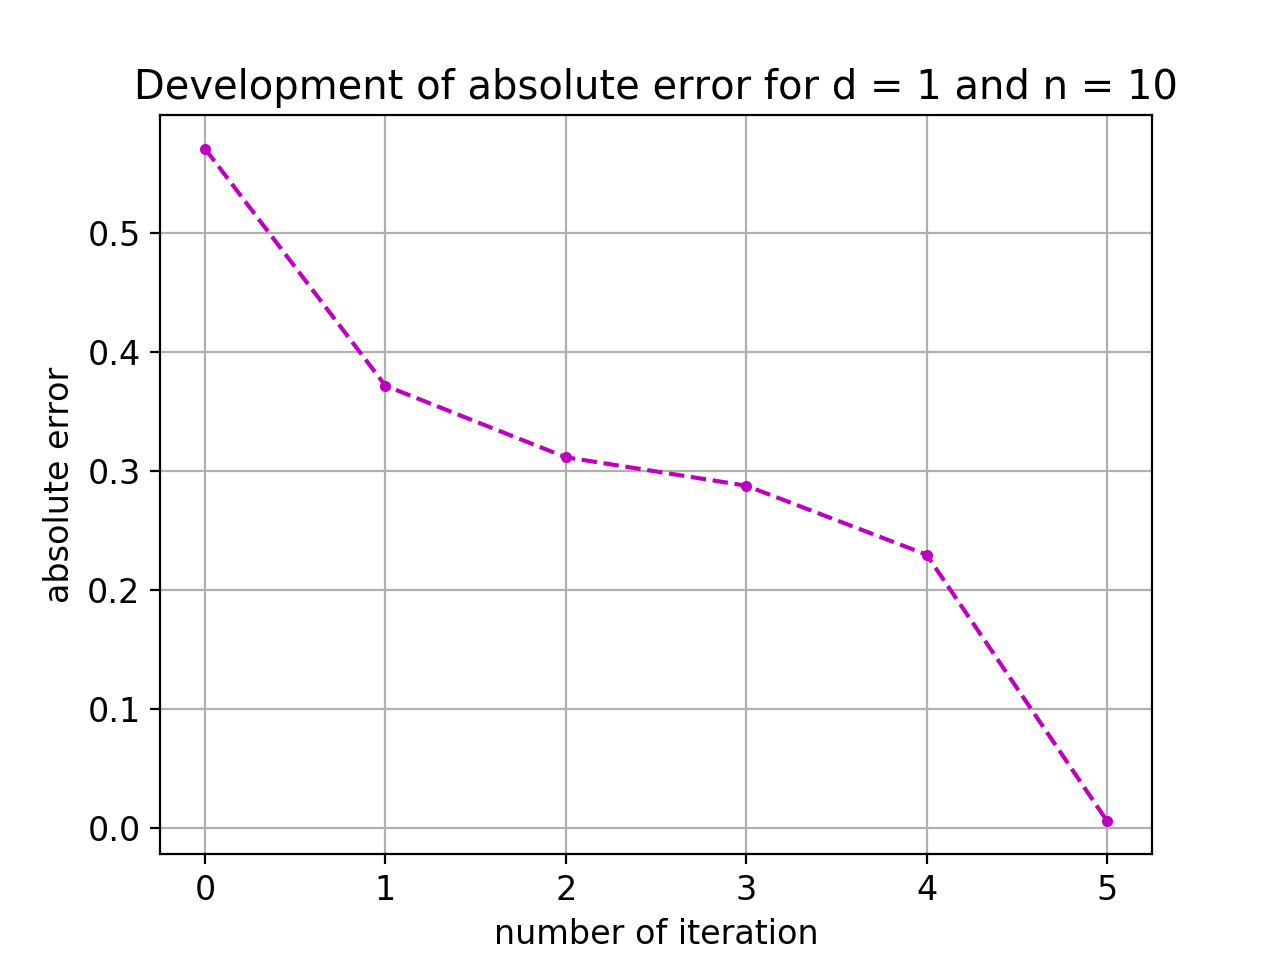
\includegraphics[width=0.45\textwidth]{Grafiken/iterates_d1_n10}
    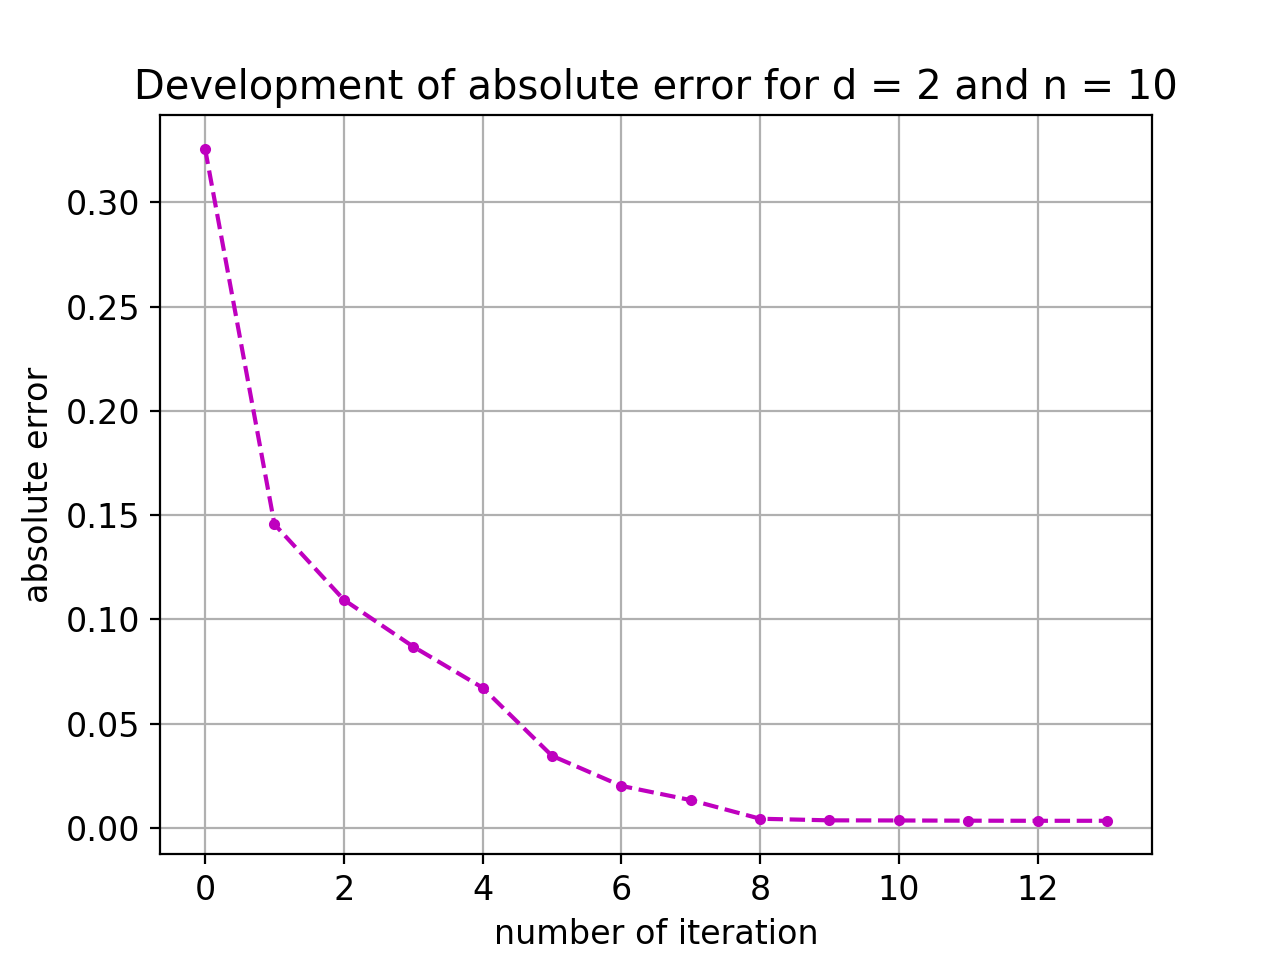
\includegraphics[width=0.45\textwidth]{Grafiken/iterates_d2_n10}
    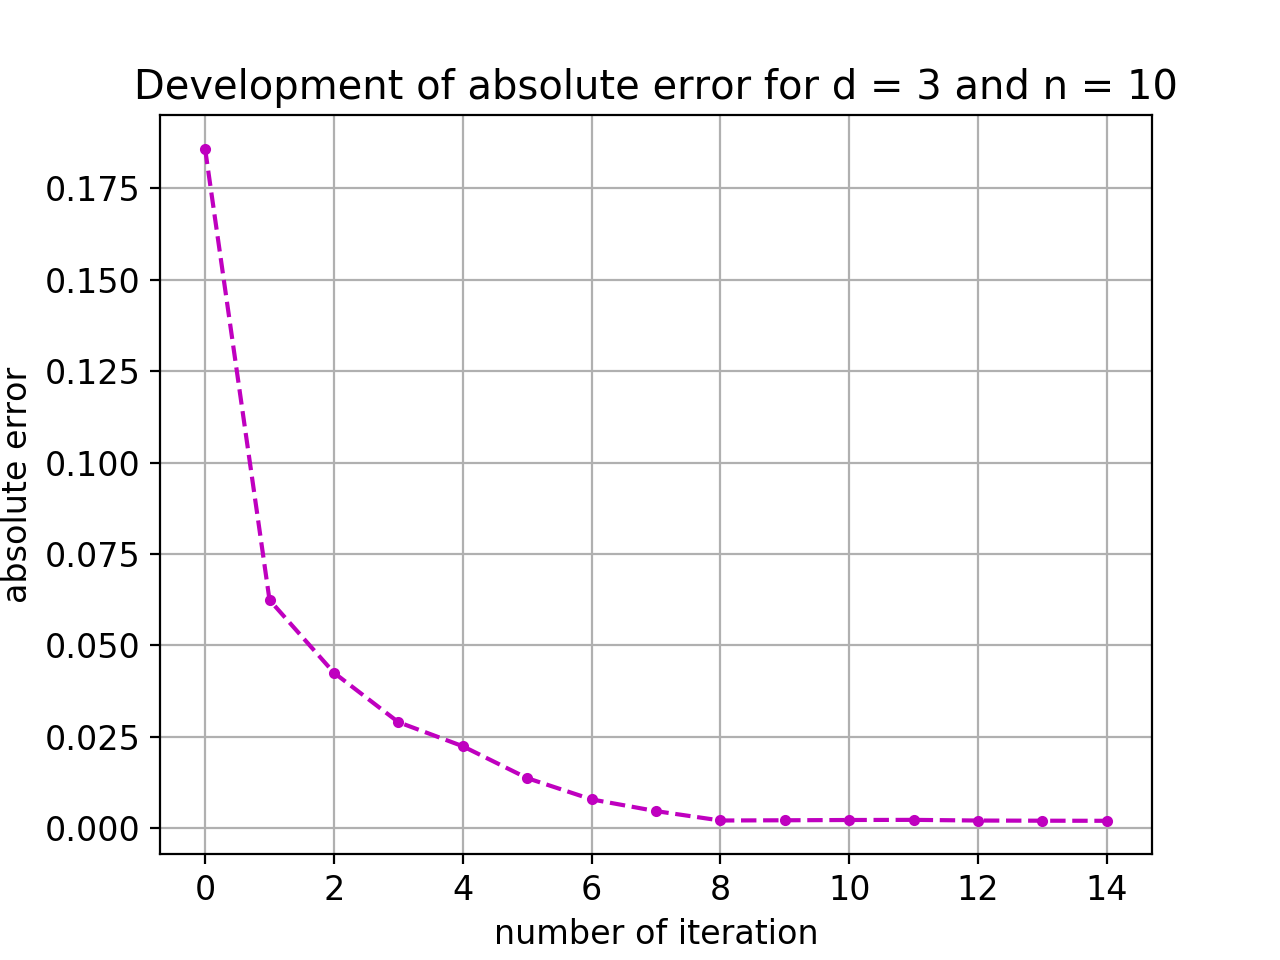
\includegraphics[width=0.45\textwidth]{Grafiken/iterates_d3_n10}
    \vspace{-0.2cm}
    \captionof{figure}{Entwicklung des absoluten Fehlers pro Iteration für $d\in\{1, 2, 3\}$ und $n=10$}
}
\vspace{0.5cm}

Darüber hinaus ist auffallend, dass weitaus weniger als $N=(n-1)^d$ Schritte vonnöten sind, um eine sehr gute Näherungslösung zu errechnen.
Während wir im eindimensionalen Fall, $N=9$, bereits nach der fünften Iteration eine ausreichend genaue Lösung haben, benötigen wir im zweidimensionalen Fall, $N=81$, nur 13 und im dreidimensionalen Fall, $N=729$, lediglich eine mehr, nämlich 14 Iterationen.
(Die große Konvergenzgeschwindigkeit lässt sich auf die gute Kondition der tridiagonalen Blockmatrix zurückführen, die wir im vorherigen Bericht ausführlich untersucht haben.)
Doch bei allen ist der Fehler schon nach acht Schritten nur noch sehr gering.
Dass unser Programm dennoch weiterrechnet, ist dem Umstand geschuldet, dass noch keiner der eingegebenen Abbruchparameter zum Tragen kam.
Da die Rechenschritte bei direkten Verfahren wie gesagt im Voraus bekannt und begrenzt sind, bei iterativen jedoch nicht, benötigen letztere Abbruchbedingungen, die den Schleifendurchlauf des Algorithmus zum Ende bringen.
Unsere Implementierung der Methode der konjugierten Gradienten (CG) enthält die folgenden drei Abbruchbedingungen.
\glqq{eps}\grqq: Abbruch, falls eine ausreichend genaue Lösung gefunden wurde, d.h. falls die Norm des Residuums eine vorgegebene Grenze unterschreitet (das Residuum, das im Bildraum von der Matrix $A$ existiert, ist ein Anhaltspunkt für die Größe des Fehlers unserer Lösung für den gesuchten Vektor $x$), \glqq{max\_iter}\grqq: Abbruch, falls der vorgenommene Aufwand ausgeschöpft wurde, d.h. falls eine vorgegebene Anzahl an Iterationen erreicht ist, \glqq{min\_red}\grqq: Abbruch, falls das Verfahren \glqq{feststeckt}\grqq, d.h. falls der Abstand zwischen den letzten beiden Residuen eine vorgegebene Grenze unterschreitet.
Dabei ist zu bemerken, dass das Greifen einer der letzten beiden Abbruchbedingungen darauf hinweist, dass das Lösungsverfahren nicht so funktioniert, wie es soll.
Daraufhin könnte man seine Eingabe eines Startwertes oder der Feinheit korrigieren oder u.U. auf eine ganz andere Methode zurückgreifen.


\subsection{Konvergenzverhalten für ein festes Epsilon}
Um den Unterschied zwischen der direkten Methode mittels Gauß-Algorithmus mit LU-Zerlegung und dem CG-Verfahren zu untersuchen, erschien es uns sinnvoll, das Konvergenzverhalten beider gegenüberzustellen.
Dieser Vergleich ist in der folgenden Grafik (Abbildung 2) für ein festes Epsilon $\epsilon = 10^{-8}$ (Abbruchbedingung 1: eine ausreichend genaue Lösung wurde gefunden) dargestellt.
Als Vektornorm haben wir die Maximumsnorm gewählt. \\
Es lässt sich beobachten, dass das direkte und das iterative Verfahren für den ein-, den zwei- und den dreidimensionalen Fall das exakt selbe Konvergenzverhalten aufweisen.
Der Gauß-Algorithmus mit LU-Zerlegung und das CG-Verfahren stellen lediglich Lösungsverfahren zur Lösung eines linearen Gleichungssystems bereit.
Die Methode zur Lösung des Poisson-Problems aber basiert in beiden Fällen auf einer Diskretisierung des Gebietes und des Laplace-Operators.
Da die Konvergenzgeschwindigkeit sowohl beim LU- als auch beim CG-Verfahren abhängig von dieser Diskretisierung ist, ist eine gleiche Konvergenzgeschwindigkeit auch nicht verwunderlich.
Noch immer gilt die Faustregel: Je feiner wir das Gitter wählen, desto genauer ist unsere numerische Lösung.
Aufgrund der zweiten finiten Differenz liegt im eindimensionalen Fall quadratische Konvergenz, im zweidimensionalen Fall lineare und im dreidimensionalen Fall sublineare Konvergenz vor. \\


{
  \centering
    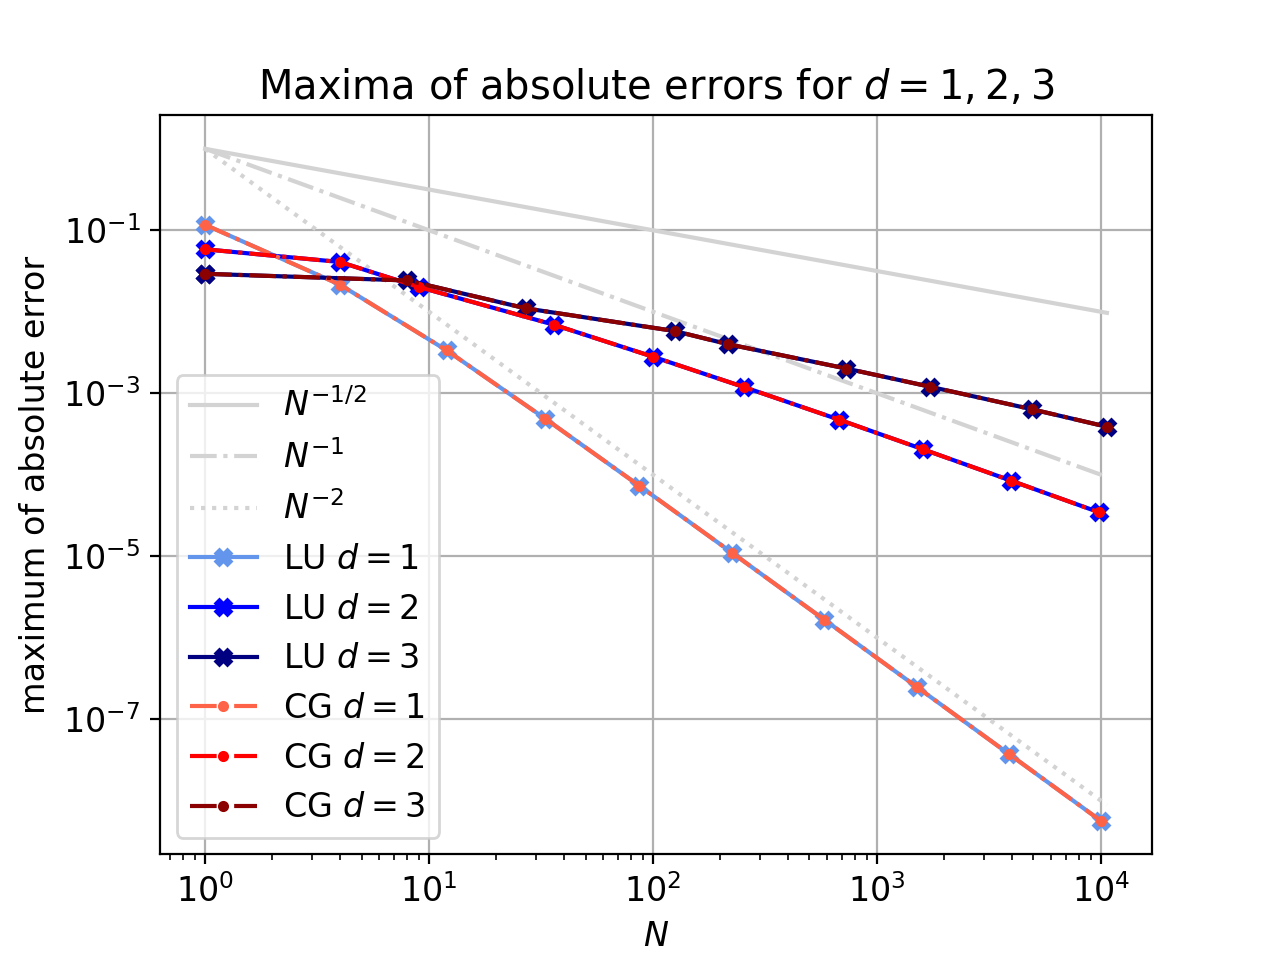
\includegraphics[width=0.75\textwidth]{Grafiken/compare}
    \vspace{-0.2cm}
    \captionof{figure}{Vergleich Konvergenzverhalten LU und CG mit $\epsilon = 10^{-8}$ für $d\in\{1, 2, 3\}$}
}
\vspace{0.5cm}


\subsection{Konvergenzverhalten für variable Epsilon}
Im Folgenden wollen wir das Konvergenzverhalten des CG-Verfahrens für eine Variation von Epsilon-Werten, die von der Feinheit der Diskretisierung abhängig ist, untersuchen.
Es gilt $\epsilon^{(k)}=n^{-k}$, wobei $n$ (mit $n \geq 2$) wie bisher die Anzahl der Diskretisierungsintervalle in je einer Dimension $d\in\{1, 2, 3\}$ angibt. \\
In der folgenden Abbildung 3 haben wir das Konvergenzverhalten für die drei untersuchten Dimensionen und die Variation der Epsilon-Werte grafisch dargestellt.
Grundsätzlich ist zu sehen, dass sich der Anstieg der Fehlerkurven mit zunehmendem $k$ immer weiter im Negativen vergrößert. \\
Für $k=-2$ und $k=0$ ist $\epsilon^{(k)}\geq 1$.
Dies bedeutet, dass das Verfahren bereits nach sehr wenigen Schritten abbricht, weil die Norm des Residuums schnell dieser Bedingung genügt.
Wir erhalten in diesen Fällen eine relativ grobe Approximation der exakten Lösung, die sich mit einer feineren Diskretisierung nicht verbessern lässt, sondern langsam immer schlechter wird (für die drei betrachteten Dimensionen mit etwa gleich großem Anstieg).
Diese Verschlechterung ist auf die zunehmenden Rundungsfehler zurückzuführen. \\
Für $k>0$ wird mit immer größerem $n$ bzw. $N=(n-1)^d$, d.h. mit einer immer feineren Diskretisierung hingegen eine Straffung der Abbruchbedingung bewirkt.
(Der Grad der Straffung hängt dabei von der Größe von $k$ ab.)
Daher sind die zugehörigen Graphen streng monoton fallend.
Das bedeutet, dass der maximale absolute Fehler immer geringer wird.
Für alle drei Dimensionen gilt, dass im Minimum für $k\geq4$ in etwa dasselbe Konvergenzverhalten wie für $\epsilon = 10^{-8}$ zu beobachten ist.
Daraus lässt sich schließen, dass $\epsilon = 10^{-8}$ eine durchaus geeignete Wahl für die Abbruchbedingung (Obergrenze Maximumsnorm des Residuums) darstellt.
Für kleinere Dimensionen allerdings genügen u.U. bereits kleinere Werte für Epsilon.
Die Wahl eines passenden Wertes ist dabei immer auch abhängig von der Größe des linearen Gleichungssystems, welche wiederum von der Größe der Dimension und der Feinheit der Diskretisierung bedingt wird. \\


{
  \centering
    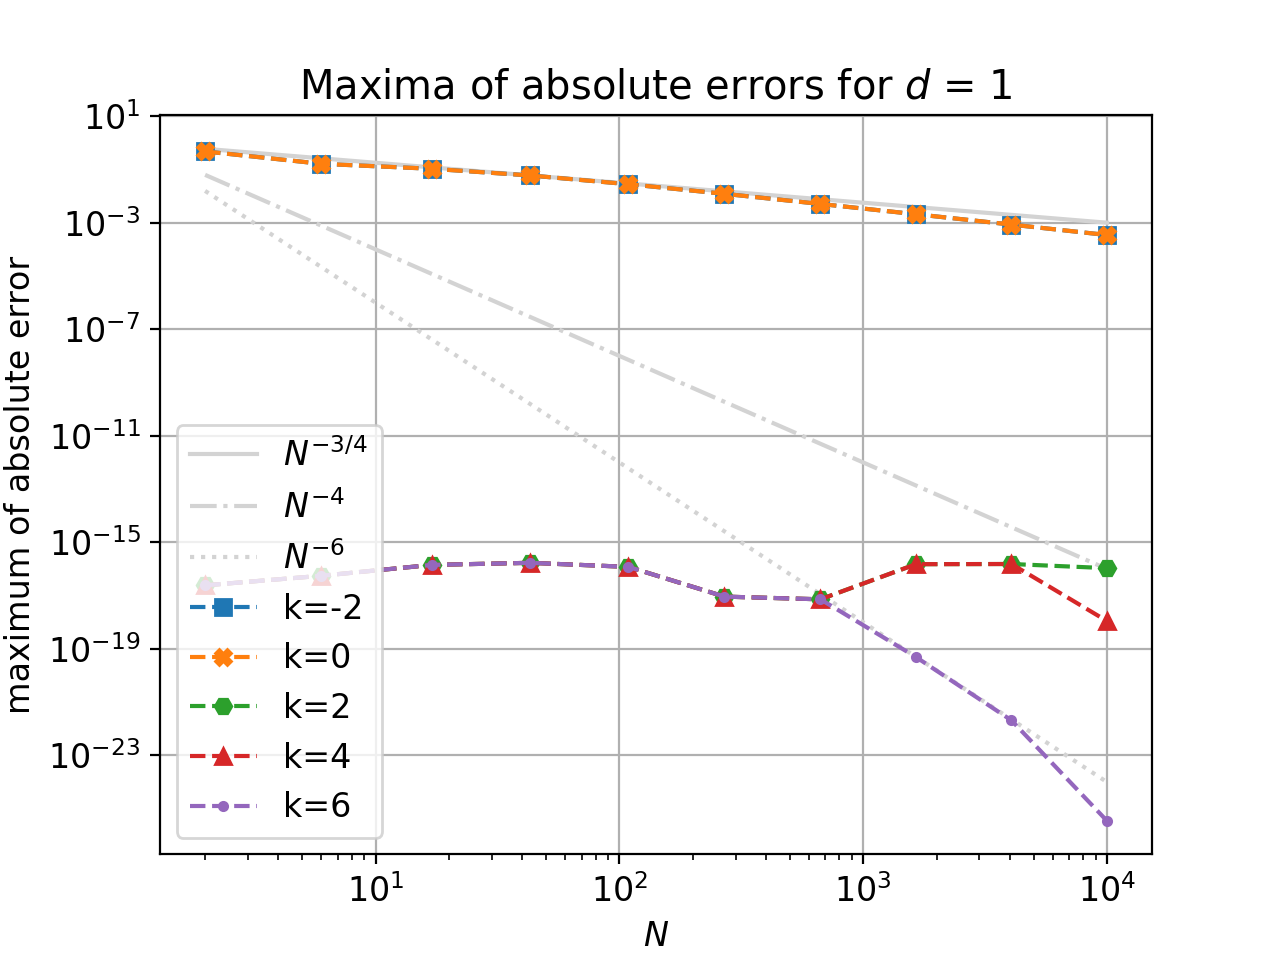
\includegraphics[width=0.45\textwidth]{Grafiken/epsilon_d1}
    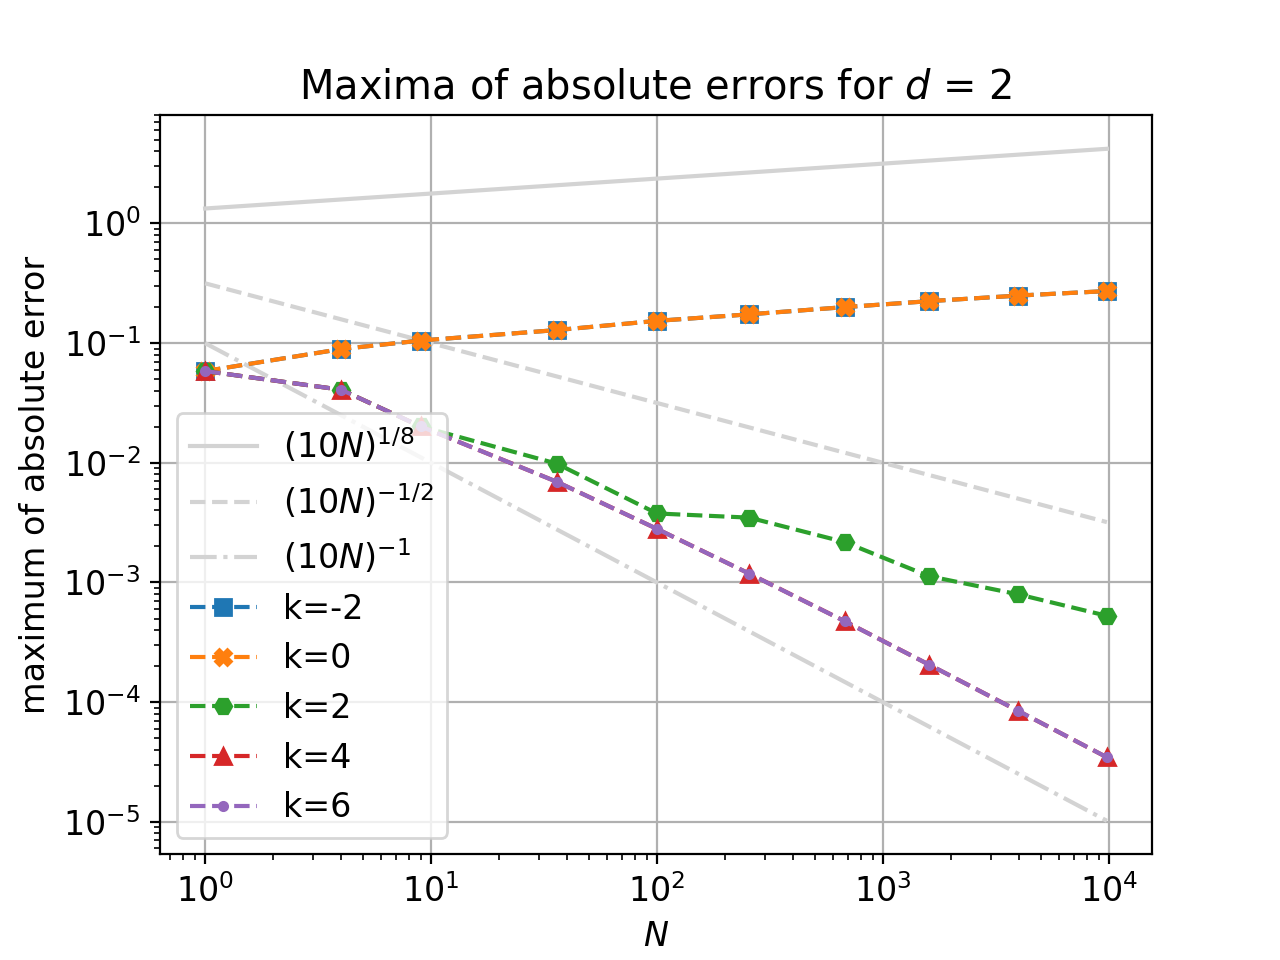
\includegraphics[width=0.45\textwidth]{Grafiken/epsilon_d2}
    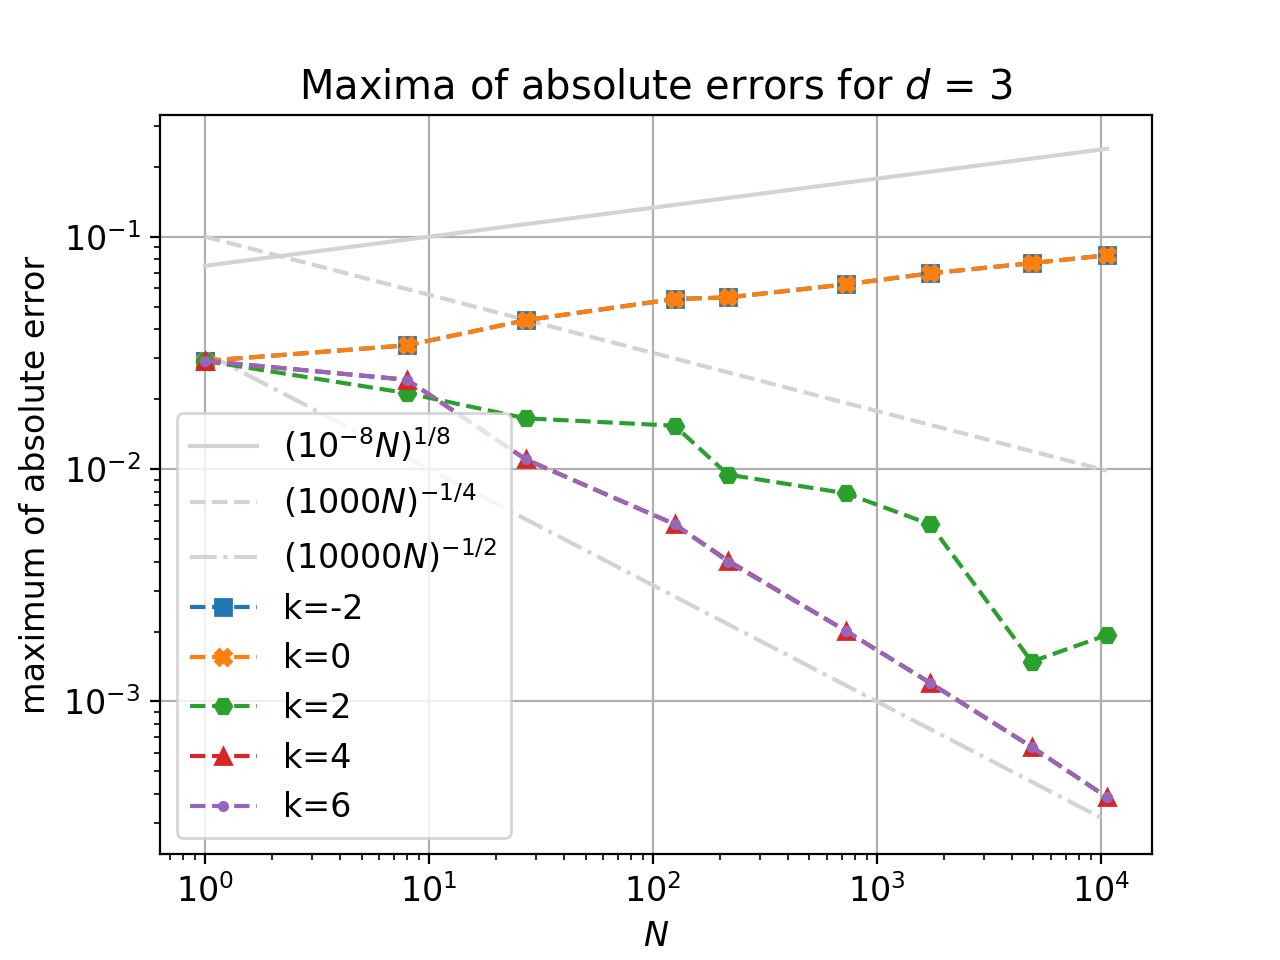
\includegraphics[width=0.45\textwidth]{Grafiken/epsilon_d3}
    \vspace{-0.2cm}
    \captionof{figure}{Konvergenzverhalten mit $\epsilon^{(k)}=n^{-k}$ für $d\in\{1, 2, 3\}$}
}
\vspace{0.5cm}


\pagebreak
\section{Abschließende Worte}
Das Lösen des Poisson-Problems mittels Finite-Differenzen-Diskretisierung produziert eine dünn besetzte Blockmatrix großer Dimension.
Möchte man dieses große Gleichungssystem mittels eines direkten Verfahrens wie dem Gauß-Algorithmus mit LU-Zerlegung lösen, würde der Speicherplatzbedarf und der Rechenaufwand durch das Erzeugen neuer Nicht-Null-Elemente rasch ansteigen.
Dadurch wäre auch eine Verfeinerung der Diskretisierung stark begrenzt.
Iterative Verfahren -- wie das in dieser Arbeit vorgestellte CG-Verfahren -- hingegen arbeiten mit Algorithmen, die die Matrix nicht verändern.
Folglich sind sie deutlich anspruchsloser hinsichtlich des Speicherplatzbedarfs.
Darüber hinaus kommen sie auch mit weniger aufwendigen Rechenoperationen aus, bieten wiederum ebenso weniger Möglichkeiten, Fehler zu produzieren bzw. sich fortpflanzen zu lassen.
Während direkte Verfahren ständig Zwischenergebnisse produzieren und damit weiterrechnen (z.B. bei der Vorwärts-/Rückwärtseliminierung), fangen iterative Verfahren diese Fehler sozusagen auf, indem sie im schlimmsten Fall lediglich mehr Zeit benötigen, um eine ausreichend genaue Näherungslösung liefern zu können.
Die Güte der Approximation wird dadurch aber nicht beeinträchtigt. \\
Durch unsere Experimente haben wir gezeigt, dass das Lösen des Poisson-Problems mittels Finite-Differenzen-Diskretisierung und Gauß-Algorithmus mit LU-Zerlegung einerseits und CG-Verfahren andererseits dieselbe Konvergenzgeschwindigkeit aufweist.
An dieser Stelle bietet also keines der vorgestellten Verfahren (LU und CG) einen Vorteil gegenüber dem jeweils anderen.
Allerdings wurde durch unsere Untersuchungen deutlich, dass beim CG-Verfahren weniger aufwendige und anfällige Rechenoperationen durchgeführt werden müssen.
Bei dem Verfahren mit der LU-Zerlegung müssen Matrix-Vektor-Multiplikationen vorgenommen werden (mit i.A. nicht mehr dünn besetzten Matrizen; die Nicht-Null-Einträge der Matrizen $L$ und $U$ addieren sich in etwa zum Quadrat der Dimension $N$ der Blockmatrix $A$), zudem müssen lineare Gleichungssysteme gelöst werden.
Beim CG-Verfahren dagegen fallen zwar auch Matrix-Vektor-Multiplikationen an, jedoch nur mit der dünn besetzten Ausgangsmatrix.
Die \textit{sparsity} der tridiagonalen Blockmatrix wird demzufolge gut ausgenutzt.
Den Rest der Operationen bilden einfache Multiplikationen von Skalaren und Vektoren.
Gleichungssysteme müssen gar nicht gelöst werden.
In der Praxis liegen vor allem sehr großdimensionale Probleme vor (auch bedingt durch die Feinheit der Diskretisierung), weshalb dieser Aufwandsunterschied stark ins Gewicht fällt.
Ein Plus, das direkte Verfahren gegenüber iterativen haben, ist der vergleichsweise geringe Zusatzaufwand bei Gleichungssystemen mit mehreren rechten Seiten.
Für diesen Fall sind iterative Verfahren demnach weniger gut gewappnet. \\
Zusammenfassend lässt sich sagen, dass das in dieser Arbeit untersuchte CG-Verfahren gut für dünn besetzte Matrizen, wie beim hier betrachteten Poisson-Problem produziert, geeignet ist.
Der Algorithmus ist stabil und stellt selbst für sehr große Systeme in nur wenigen Rechenschritten eine gute Approximation der exakten Lösung bereit. 


\pagebreak
\bibliographystyle{plain}
\bibliography{serie5_literatur}

\end{document}
